

\pgfdeclarelayer{bg}
\pgfsetlayers{bg,main}


\begin{figure}
    \centering
    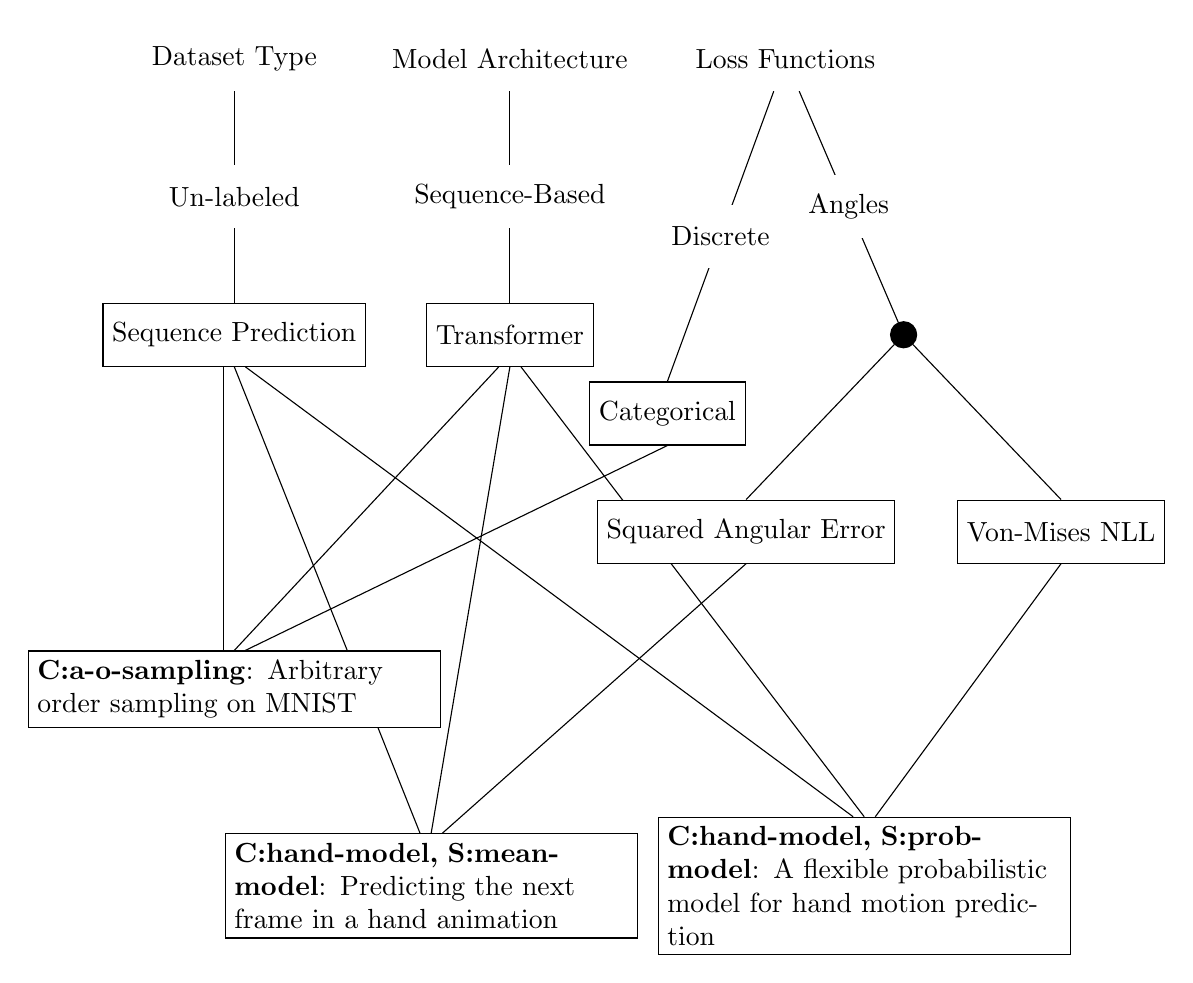
\begin{tikzpicture}
        \tikzstyle{every node}=[node distance=3.5cm,minimum height=0.8cm]

        % dataset type
        \node (datasettype) {Dataset Type};
        \node[draw, below of=datasettype] (seqpred) {Sequence Prediction};
        \draw (datasettype) -- node[fill=white] {Un-labeled} (seqpred);

        % input shape
        \node[right of=datasettype] (seqmodel) {Model Architecture};

        % loss
        \node[right of=seqmodel] (loss) {Loss Functions};

        % angles
        \node[draw,fill=black,minimum height=0.2cm,circle,below of=loss,xshift=1.5cm] (angles) {};
        \draw (loss) -- node[fill=white] {Angles} (angles);

        \node[draw,fill=white,below of=angles,node distance=2.5cm, xshift=-2cm] (amse) {Squared Angular Error};
        \draw (angles) -- (amse.north);

        \node[draw,fill=white,below of=angles,node distance=2.5cm, xshift=2cm] (vonmises) {Von-Mises NLL};
        \draw (angles) -- (vonmises.north);

        \node[draw,fill=white,below of=loss,node distance=4.5cm,xshift=-1.5cm] (cat)  {Categorical};
        \draw (loss) -- node[fill=white] {Discrete} (cat.north);

        % transformer (here because needs to draw above a line)
        \node[draw, below of=seqmodel] (transformer) {Transformer};
        \draw (seqmodel) -- node[fill=white] {Sequence-Based} (transformer);


        % chapter 4: arbitrary order sampling
        \node[draw,fill=white,text width=5cm] (chapter4) at (0,-8cm) {\textbf{\Cref{C:a-o-sampling}}: Arbitrary order sampling on MNIST};

        % chapter 6.2: transformer for hand pose prediction
        \node[draw,fill=white,text width=5cm] (chapter62) at (2.5cm,-10.5cm) {\textbf{\Cref{C:hand-model}, \Cref{S:mean-model}}: Predicting the next frame in a hand animation};

        % chapter 6.3: probabilistic model for hand pose prediction
        \node[draw,fill=white,text width=5cm] (chapter63) at (8cm,-10.5cm) {\textbf{\Cref{C:hand-model}, \Cref{S:prob-model}}: A flexible probabilistic model for hand motion prediction};

        \begin{pgfonlayer}{bg}
            \draw ([xshift=-4pt]seqpred.south) -- ([xshift=-4pt]chapter4.north);
            \draw ([xshift=-4pt]transformer.south) -- (chapter4.north);
            \draw (cat.south) -- ([xshift=4pt]chapter4.north);

            \draw (seqpred.south) -- ([xshift=-4pt]chapter62.north);
            \draw (transformer.south) -- (chapter62.north);
            \draw (amse.south) -- ([xshift=4pt]chapter62.north);

            \draw ([xshift=4pt]seqpred.south) -- ([xshift=-4pt]chapter63.north);
            \draw ([xshift=4pt]transformer.south) -- (chapter63.north);
            \draw (vonmises.south) -- ([xshift=4pt]chapter63.north);
        \end{pgfonlayer}

    \end{tikzpicture}
    \vspace{1cm}
    \captionsetup{parskip=7pt}
    \caption[Where my work sits.]{The later work in this thesis sits focuses on learning un-labeled sequence data with transformers, in two different domains.

    In \Cref{C:a-o-sampling}, I train a transformer-based probabilistic model which can be used as a gaussian process for predicting pixels on the MNIST dataset.

    In \Cref{C:hand-model}, I train a transformer-based model on the ManipNet hand motion dataset. \Cref{S:mean-model} focuses on a deterministic model, while \Cref{S:prob-model} focuses on a probabilistic model.}
    \label{fig:context}
\end{figure}
